\chapter{Discussion}
\label{chap:discussion}
% - Start off comparing basic stuff like masses and radii of your disks, so that we get the idea that relative to large populations of disks they are big and dense, but that relative to Sam’s disk they are comparable in mass/radius.



With the disks now fit, we may interpret our results. Since this project was framed around the question of how environment influences protoplanetary disks, we would like to compare our best fit values to other disks, including to one other from the ONC \citep{Factor2017} as well as to others outside of it. We begin with a brief review of the relevant literature on the three disk features that we fit (densities, temperatures, and chemical abundances) so that we may frame our results in a meanigful context.







\section{Physical Structure}


% REWORK: One thing you need to make sure to include in any discussion of disk mass ranges is a discussion of sensitivity limitations.  Are there disks with masses less than 1 M_Jup?  Probably!  Are they detectable?  Nope.  Also, the sensitivity limits are lower for low-mass SF regions than for high-mass, simply because they’re closer, which is another important caveat that is currently missing from your discussion. 



To get a sense of how these disks' physical characteristics (i.e. mass and radius) compare to other protoplanetary disks, it is useful to compare our results to other disks in the Orion Nebula Cluster, as well as others in low-mass star forming regions (SFRs). It is worth again reiterating that many of the reported disk gas masses in the literature \citep[as well as the value we use here from][]{Williams2014} are calculated from continuum emission (which traces dust mass), and then scaled by the factor of 100 to return a gas mass. However, as briefly discussed in \S\ref{chap:introduction}), this ISM-based gas/dust ratio has been shown to be neither constant across surveys disks nor best approximated by 100:1.


In an attempt to avoid relying on the use of the 100:1 gas/dust ratio, \citet{WilliamsBest2014} presented a method to infer a disk's gas mass by comparing ratios of CO isotopologues. The method they present involves developing parametric disk models over a wide range of parameters (similar to the modeling process that we use) and calculating the resulting emission intensities of selected lines (generally C$^{18}$O and $^{13}$CO due to their relative abundances but lack of cloud contamination). By generating a large set - or ``grid" - of models over a range of parameter values, observations of a disk can then be located on that grid, essentially through template fitting. In this process, they hold certain molecular and atomic abundance ratios fixed (most notably, their CO/H$_2$ ratio is held at the molecular cloud-level of 10$^{-4}$). Their application of the method to nine well-studied disks in Taurus yielded masses appreciably lower than a 100:1 gas/dust ratio would have implied, instead returning a wide range of ratios that were centered around 10:1. Analysis of 89 disks in Lupus \citep{Ansdell2016} using this method also showed a similar trend, although due to insufficient C$^{18}$O detections, only 11 of the disks' masses were able to be fully estimated, while another 25 had upper limits established.

\citet{Miotello2014}, \citet{Miotello2016} and \citet{Miotello2017} build on the methods of \citet{WilliamsBest2014}, using CO isotopologue ratios to find gas mass, but avoid the use of fixed abundance ratios by integrating a full chemical-reaction network to reflect the effects of freeze-out and photodissociation (the two main effects driving chemical evolution), allowing the abundance ratios to self-equilibrate. With this addition, they were able to reanalayze and expand the sample of constrained gas masses from the \citet{Ansdell2016} survey from 11 to 34. Their results again show that the use of a fixed gas/dust ratio is inappropriate, and that 100:1 is typically far too high. \citet{Miotello2017} notes that this deficiency could be the result either of an actual lack of gas, or could reflect a high rate of carbon depletion (through chemical evolution, locking-up in larger bodies, or loss of gas), but that these observations are insufficient to discern between them.

% \textit{Could cite Bergin+ 2013 here for coming up with the HD stuff, but not sure how to make it work narratively.}

% REWORK: Maybe good to include discussion of Ansdell2017? Survey of 92 disks in sigOri, only 6 CO detections, use a comb of Williams and Best/Miotello methods.

\begin{figure}[ht]
  \hspace*{\fill}%
  \subcaptionbox{}{\includegraphics[width=0.8\linewidth]{Miotello17_GDR_hist.png}}\vfill%
  \subcaptionbox{}{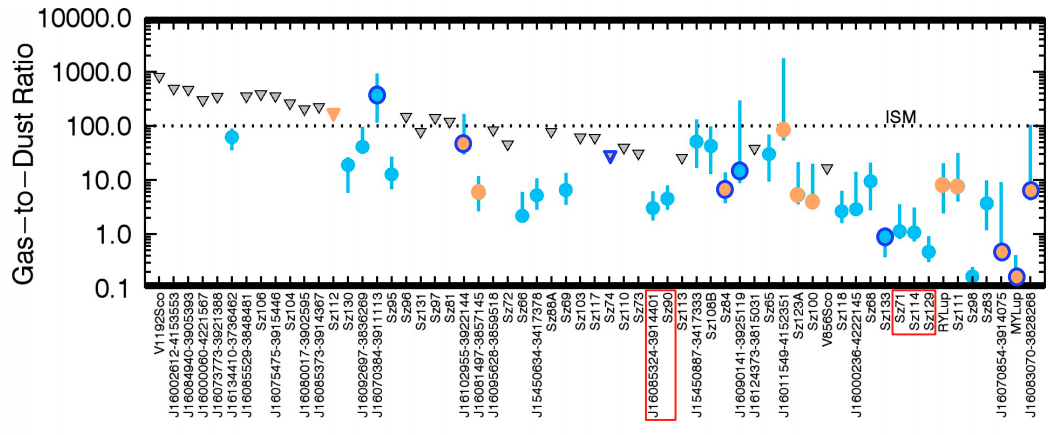
\includegraphics[width=\linewidth]{Miotello17_GDRs.png}}%
  \hspace*{\fill}%
  \caption{blah balh}
  \label{fig:GDRs}
\end{figure}


When calculating gas masses for the disks in d253-1536, \cite{Williams2014} found the disks' total dust masses from continuum emission and used the 100:1 gas/dust ratio discussed above to infer the gas masses. The uncertainty that this introduces, as well as the uncertainty from the actual flux measurement (noted in \S\ref{chap:results}), is crucial to keep in mind, as these factors imply that the resulting gas masses are possibly up to an order of magnitude or two too large. A table of the disks' masses and radii, as well as those from \citet{Factor2017}, are presented in Table \ref{table:disk_masses_rads} for reference throughout this chapter.


% Not sure if this table is a good idea.
\begin{table}[ht!]
  \centering
  \begin{threeparttable}
    \caption{Disk Parameter List}
    \label{table:disk_masses_rads}
    \renewcommand{\arraystretch}{1.2}
    \begin{tabular}{l c c c c c c}
      \toprule \toprule
      %\multirow{2}{*}{Parameter} & \multirow{2}{*}{Disk A}    & \multicolumn{2}{c}{Disk B} \\
      \multirow{2}{*}{Disk}  & Radius\tnote{a} & Radius\tnote{b} & \multicolumn{2}{c}{Gas Mass\tnote{c}} &  Dust Mass\tnote{d} \\
                             & (au)            & (au)            & (M$_\odot$)       & (M$_\text{Jup}$)  & (M$_\oplus$)  \\
      \midrule %\midrule
      d253-1536a             & 340             & 268             & $7.5 \times 10^{-2}$        & 78.66   & 250   \\
      d253-1536b             & 148             & [-]             & $2.9 \times 10^{-2}$        & 29.88   & 95     \\
      d216-0939              & 530             & 525             & $4.4 \times 10^{-2}$        & 45.84   & 145   \\
      \bottomrule
    \end{tabular}
    \begin{tablenotes}\footnotesize
      \item[a] Results of MCMC fitting of \hco emission.
      \item[b] Semi-major axis of 2D Gaussian fit to the disk's continuum emission \citep{Mann2014}
      \item[c] \citet{Williams2014}
      \item[d] Since \citet{Williams2014} use a 100:1 gas/dust ratio, we may infer the dust emission to be two orders of magnitude lower than the gas.
    \end{tablenotes}
  \end{threeparttable}
\end{table}



% REWORK: Maybe add a sensitivity limit.
With this in mind, we can compare these disks' masses and radii to others. The natural place to start for this is with the survey of ONC proplyds that originally provided these data \citep{Mann2014}. In it, the authors infer total disk masses and fit the disks with 2D elliptical Gaussians, and using the resulting semi-minor and -major axes of the disks as approximate measures of the disks' radial extents. Disk A in the present system was, by their measure, the most massive disk in the study, 75\% ($37\sigma$) more massive than the study's next most massive disk, d216-0939 \citep[which was the subject of][]{Factor2017}; disk B was the fifth most massive. Disk A had the study's fourth largest semi-major axis\footnote{The authors' measurement of disk A's semi-major axis, at 268 au, is $2.6\sigma$ smaller than our fit measurements. The survey's reported semi-major axis for d216-0939 was also smaller than the fit value in \citet{Factor2017}, though by less than $1\sigma$. This probably reflects something about how we define gas/dust outer radii REWORK see how surf dens is implemented, and Hughes2008}. The authors did not fit disk B's radial extent; however, our fit for its radius would make it the eleventh (out of 22) largest disk in the survey. Thus, disk A is on the very high end of the study's mass and radius range, while disk B is apparently quite dense and of median radial extent.



This work was followed by a survey of 104 detected disks in the heart of M42 within 0.14 pc of $\theta^1$ Ori C \citep{Eisner2018}. The authors measure the disks' dust masses (from continuum flux) and radii (again from fitting 2D elliptical Gaussians), and compare their distributions to similar measurements from other surveys of disks in low mass SFRs. These comparisons are summarized in Fig. \ref{fig:eisner18_disk_properties} (see figure caption for references), showing the distributions of masses and radii of disks in each survey. From them, we see that these M42 disks are characteristically denser and radially truncated, as shown by the ONC track's relatively high position on the mass plot and relatively low position on the radius plot. By locating our two disks on these plots, we find that their dust masses are far greater than the M42 disks and that disk A is more massive than any of the disks in all the surveys. However, while the ONC disks in this plot exhibit an atypically high density (the highest-mass disks have mass/radius ratios of around 1.5 M$_\oplus$/au) relative to the other survey's disks (which are closer to of order 0.5 M$_\oplus$/au), disk A and B land at 0.75 and 0.65, respectively. This indicates that, while they are still somewhat more dense than the disks from low-mass SFRs, they show neither the radial truncation nor high densities found in the M42 disks.

% REWORK: Feels real awkward to put this here, idk.
% A survey of dust masses for 279 disks in $\rho$ Ophiuchus by \citet{Williams2019} found that the regions's disk population had masses systematically slighter below those in Lupus \citep[][; shown in blue in Fig. \ref{fig:eisner18_disk_properties}]{Ansdell2017} but functionally similar.



% REWORK: Get survey refs
\begin{figure}[h!]
  \centering
    \hspace*{\fill}%
    \subcaptionbox{Disk mass distribution across surveys}{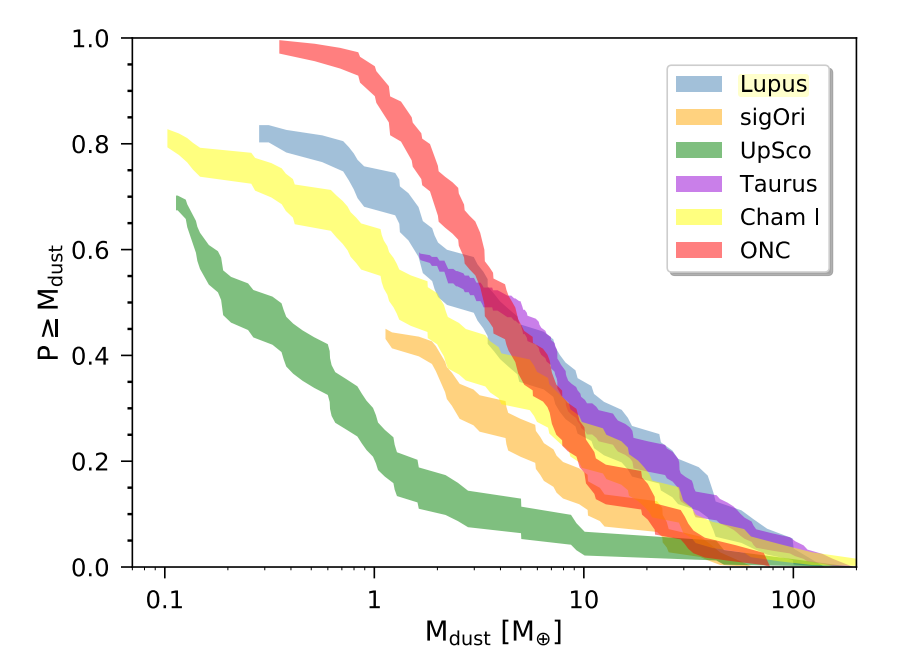
\includegraphics[width=0.5\linewidth]{dust_mass_dist_Eisner18.png}}%
    \subcaptionbox{Disk radius distribution across surveys}{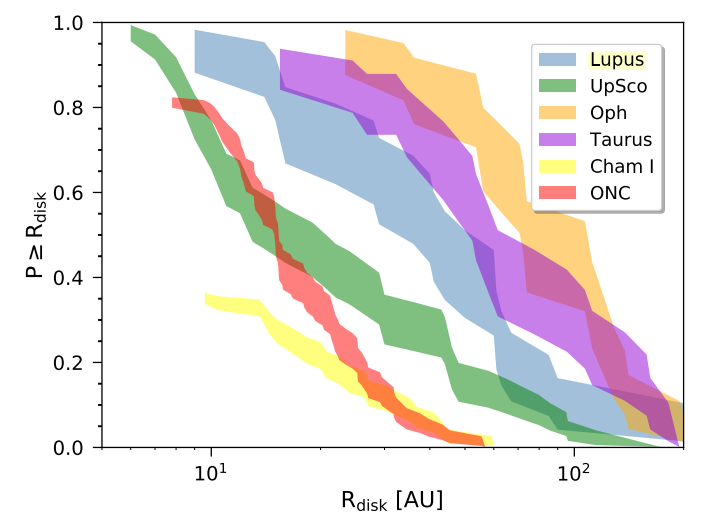
\includegraphics[width=0.5\linewidth]{dust_radius_dist_Eisner18.png}}%
    \hspace*{\fill}%
    \caption{Comparing the distribution of masses and radii across surveys of different regions \citep{Eisner2018} reveals that, while disks in the ONC have disk masses comparable to those of other regions, their radii are systematically truncated. \textit{Survey References:} Lupus: \citet{Tazzari2017}; $\sigma$ Ori: \citet{Ansdell2017}; Upper Sco: \citet{Barenfeld2017}; Taurus \& Ophiucus: \citet{Tripathi2017}; Cham 1: \citet{Pascucci2016}}
    \label{fig:eisner18_disk_properties}
\end{figure}


% REWORK: These "low" masses correspond to numbers way bigger than anything in those plots.
It is also worth noting that by using the methods described above to measure gas masses directly, \citet{Miotello2017} found no disks more massive than 1.6 M$_\text{Jup}$, while \citet{Ansdell2016} and \citet{Ansdell2018} found masses reaching no higher than 10 M$_\text{Jup}$.


With the results of these surveys as context, we see that the disks in the d253-1536 binary have large radii and that their reported masses are extremely large, yielding densities that are higher than disks in low-mass SFRs but not as high as others in the ONC. However, due to the uncertainty in the mass measurement (both from the assumed gas/dust ratio and the uncertainty in locating the edges of each disk due to their overlap), the masses could be significantly less massive than reported. It is also possible that they could be more massive (and dense) than their reported values, but since both sources of uncertainty show trending towards under-estimation \citep[][showed that disks in Lupus were better represented by a 10:1 gas/dust ratio, and, as discussed in \S\ref{chap:results}, the integrated flux measurement that yields the disks' dust masses is likely over-counting emission]{Miotello2017}, it is more likely that these values are too high than too low.



% REWORK: Integrate this in.
\citet{Andrews2013} showed that the masses of disks in Taurus are linearly correlated with the mass of their host stars, going as M$_\text{disk} \approx 0.4$\% M$_\star$ and ranging by up to a factor of 40. Our disks have masses approximately equal to 2\% and 7\% of their host stars for disk A and B, respectively, which is consistent with their linear fit and the associated uncertainty. There is also sufficient uncertainty in the measurement of these disks' masses - from the 100:1 gas/dust ratio and dust temperatures assumed in the mass calculation - that these values lack the precision necessary to





\subsection{Comparison to Binaries}

% T Tauri Binary surveys: Duchene1999, Kraus2008, Kraus2011

% Binaries in the ONC (2012) (not radio): https://www.aanda.org/articles/aa/pdf/2012/04/aa18314-11.pdf
% Binaries in Taurus (2012): Harris2012
% Binaries in Taurus (2019): Akeson2019
% Binaries in rho Ophiucus (2014): Akeson2014 (49 systems, 63 stars)
% Binaries in rho Ophiucus (2017): cox2017
% GG Tau A: Dutrey2014
% In close (\textless100 au) binary systems, it is predicted \citep{someone} that circumstellar disks should develop around each star in addition to an outer circumbinary disk. \citet{Dutrey2014} used high-resolution ALMA observations to reveal such a system around a heirarchical triple system (where a binary pair is one element of a larger binary) revealed complex interactions between the various disks. However, since both tiers of this system are very close (the outer binary has an apparent separation of 35 au, while the inner pair are separated by just 4.5 au), the system is not entirely comparable to our present binary.



We must also consider the fact that our disks are in a binary. While this work is not meant to be a complete review of multiple star systems \citep[for a more comprehensive review, see][]{Duchene2013}, some review of the relevant literature is warranted to frame our interpretation of the present system.

Binaries (and higher-order systems, which generally form as heirarchical pairs) are quite common, with around 30\% of low- and intermediate mass Main Sequence stars presenting with companions; that number climbs to 70\% for high mass stars \citep{Sana2012}, and surveys of younger, T Tauri stars in low-mass regions show even higher fractions, up to almost 80\% in Taurus \citep{Kraus2011}, for example. However, regions of higher densities (like the ONC) seem to have the opposite effect, as \citet{Reipurth2007} found that the 781 sources within 60'' of $\theta$ Ori C contained only 69 multiple systems (with apparent separations between 67 and 675 au), yielding to a companion fraction of just 9\%. There is notable subsetting within that population, particularly with a defiency of wide (0.''5 - 1.''5, or around 200-600 au at the ONC's Gaia-measured distance of 389 pc) binaries closer to $\theta_1$ Ori C (see Fig. \ref{onc_binary_stats}). Our binary, with an angular separation of 1.''1, represents one of the widest pairs in the ONC, and is comfortably into the ``flat'' region (at $d = 591''$) of the radial distribution of binaries from $\theta_1$ Ori C.


% REWORK: Duchene2013 p.16 says binaries are more likely to be close bc of tidal interactions between disks

% Implications of the disks' misaligned rotational axes. \citet{Lai2014} shows that it's pretty easy to make them misaligned. AkesonJensen2014 show that HK Tau is fucked up.

% REWORK: Add stuff about binary formation.
% There are two favored pathways to the formation of multiple star systems: the fragmentation of a gravitationally unstable disk \citep[e.g. ][]{Kratter2010} and turbulent fragmentation of the molecular cloud \citep{Offner2010}. Of these two pathways, it has seemed that
% A survey of 17 multiple protostar systems in Perseus with separations less than 600 au by \citet{Tobin2018} implied that disk fragmentation, rather than REWORK, is likely the dominant formation method for binary systems.

\begin{figure}[h]
  \hspace*{\fill}%
  \subcaptionbox{}{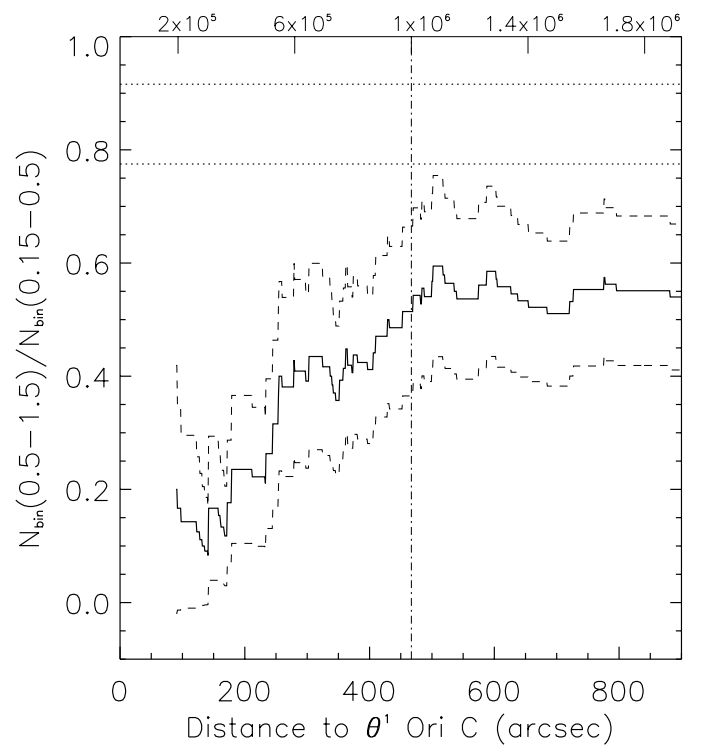
\includegraphics[width=0.5\linewidth]{Reipurth2007_binfrac_by_dist_thetaoric.png}}%
  \subcaptionbox{}{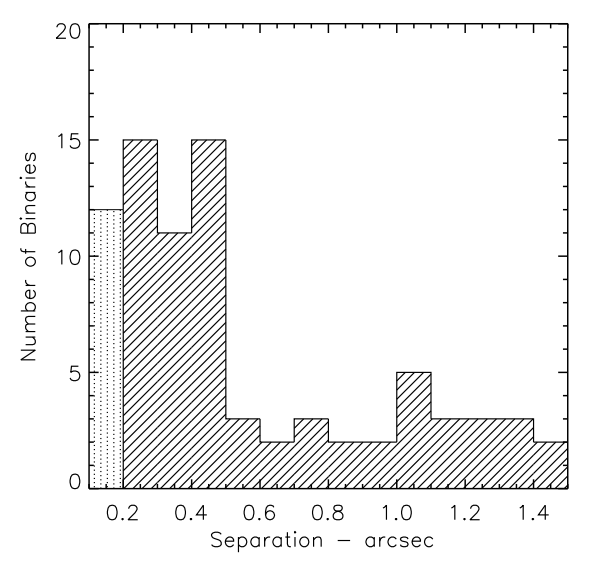
\includegraphics[width=0.5\linewidth]{Reipurth2007_binfreq_by_sep.png}}%
  \hspace*{\fill}%
  \caption{Statistics for binary pairs in the Orion Nebula Cluster \citep{Reipurth2007}. In (a), the vertical dotted line represents the point at which the distribution becomes flat. The present system is around 591'' from $\theta_1$ Ori C, putting it beyond the radius apparently affected by the massive star.}
  \label{fig:onc_binary_stats}
\end{figure}




As one might expect, disks are not uncommon around disks in binaries. Several millimeter/sub-millimeter surveys have observed a number of disks in binary systems in various regions, most notably in Taurus and $\rho$ Ophiucus. Since these regions are low-mass SFRs, they are qualitatively different environments than the ONC, but provide us with a good starting point to compare to.



\begin{figure}[h!]
  \subcaptionbox{\citet{Harris2012}}{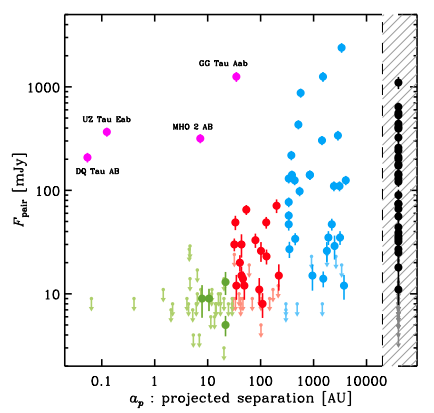
\includegraphics[width=0.5\linewidth]{harris2012_binary_brightnesses.png}}%
  \subcaptionbox{\citet{Akeson2019}}{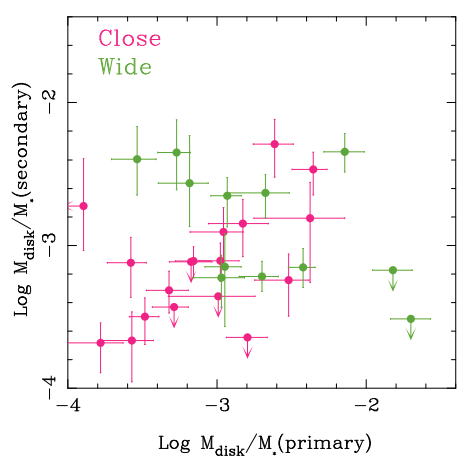
\includegraphics[width=0.5\linewidth]{akeson2019_binary_mass_ratios.png}}%
  \caption{Population trends from binary pairs in the Taurus star-forming region. ($a$): There is a clear upper limit on pair flux that is correlated to projected separation (green, red, and blue marks represent close, medium, and wide pairs). the presence of a circumbinary disk (magenta) yields an extra source of flux, and so pairs featuring such a disk do not follow the separation-limited flux pattern. ($b$): The mass of the disk around the secondary member of the binary in close systems (pink) is correlated to the mass of the primary, while in wide systems (green), the two are anti-correlated.}
  \label{fig:taurus_binaries}
\end{figure}

\begin{figure}[h]
  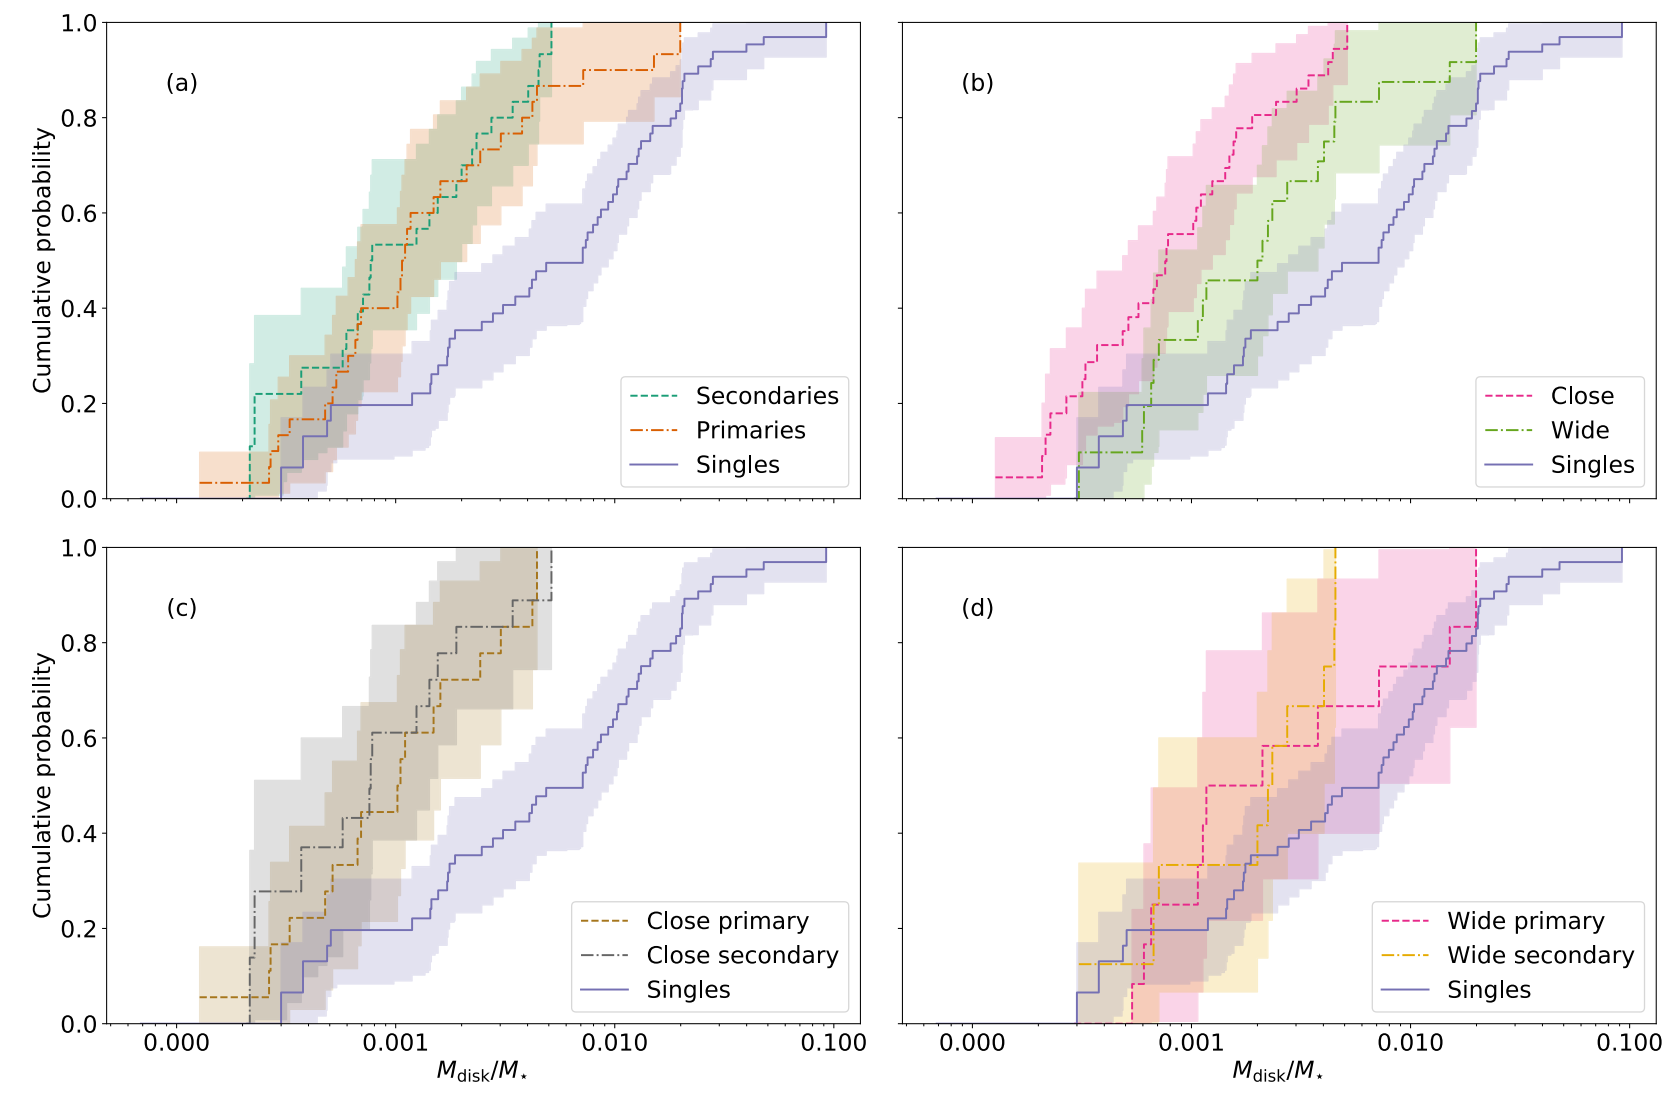
\includegraphics[width=\linewidth]{akeson2019_binary-disk-masses.png}%
  \caption{Cumulative probabilities of disk masses for different combinations of disks in binary pairs \citep{Akeson2019}. ($a$): Both disks in binary pairs are systematically less massive than single (isolated) disks although, as expected, the primary has more representation at the more massive end. ($b$): Close pairs are more significantly truncated than wide pairs, although wide pairs are still under-massive as well. ($c$) Close pairs do not preferentially truncate either disk; each has a sharp upper limit. ($d$): Primaries in wide pairs have nearly the same mass probability as single disks.}
  \label{fig:binary-disk-masses}
\end{figure}

% Not sure how to slide this in. 'It has long been known \citep[and references contained therein][]{Jensen1995} that close (\textless50-100 au) binaries have lower combined millimeter fluxes than wider binaries or single stars.'

% REWORK: the Jensen1996 reference is a PhD thesis; try to find the actual paper?
\citet{Harris2012} observed disks in 23 multiple-star systems in Taurus using the Submillimeter Array. In it, they found a strong anticorrelation between system brightness and projected separation between components, with wide pairs (\textgreater300 au) showing similar brightness to that of two single stars, while tight pairs (\textless30 au) suffer a $5\times$ decrease from the equivalent sum of individual brightnesses (although the presence of circumbinary disks around binaries of any separation make the system significantly brighter; see Fig.\ref{fig:harris2012_binary_brightnesses}). \citet{Akeson2019} built on these results with an ALMA survey of additional binaries in Taurus, developing a sample of 151 sources with resolved millimeter detections, 99 of which were in binary systems. From this sample, they found that disks around the binaries' primary (more massive) star contribute, on average, 62\% of the disks' total combined mass, although this distribution has a wide spread. They also developed the observation by \citet{Harris2012} \citep[and previously in][]{Jensen1996} that tighter binaries led to lower fluxes, finding that, as a function of stellar mass, disks in binaries have systematically lower masses than their isolated counterparts, and that this mass truncation is more apparent in tighter binaries (see Fig. \ref{fig:taurus_binaries}). They found that M$_\text{disk}$/M_$\star$ for the primary and secondary stars are correlated in close systems but anticorrelated in wide systems, and that the rough correlation between disk mass and stellar mass shown in \citet{Andrews2013} did not hold in their sample. Finally, they note that the absence of a significant population of circumbinary disks in the sample suggests that they are either not common or quickly (\textless1-2 Myr) dissipated.


% "For this sample of wide binaries, the secondary/primary disk mass ratio is not correlated with the secondary/primary stellar mass ratio. This suggests that for these binary systems, any environmental factors shared between the two components that could affect the initial disk mass and disk evolution are not the dominant factor in determining the range of disk masses for a given stellar mass." (Akeson2014)

Disks in binary pairs have also been surveyed in the $\rho$ Ophiucus region. \citet{Akeson2014} studied 17 pairs with separations ranging from 100-990 au using ALMA, measuring the systems' masses. In it, they found no correlation between disk mass and stellar masses, matching the results from the studies of Taurus binaries above. \citet{Cox2017} followed with a survey targeting 63 total sources, comprised of 11 binaries, three triple systems, and 34 single sources. In it, they, like \citet{Harris2012} and \citet{Akeson2019}, found significantly lower fluxes from sources in binaries than isolated ones, and found that the disks' radii also exhibited systematic truncation. They note that this truncation is likely either due to tidal interactions between the disks or reflects a natural limit on the radii of disks in binaries, inherent to the disks' formation process, and that these decreased fluxes can be generally interpreted as being proportional to decreased masses. They also found no correlation between the ratios of the stellar masses and the ratios of the disk masses in the sample, indicating that environmental factors that both components share are likely not a dominant factor in determining disk masses.


 \begin{figure}[h]
   \hspace*{\fill}%
   \subcaptionbox{}{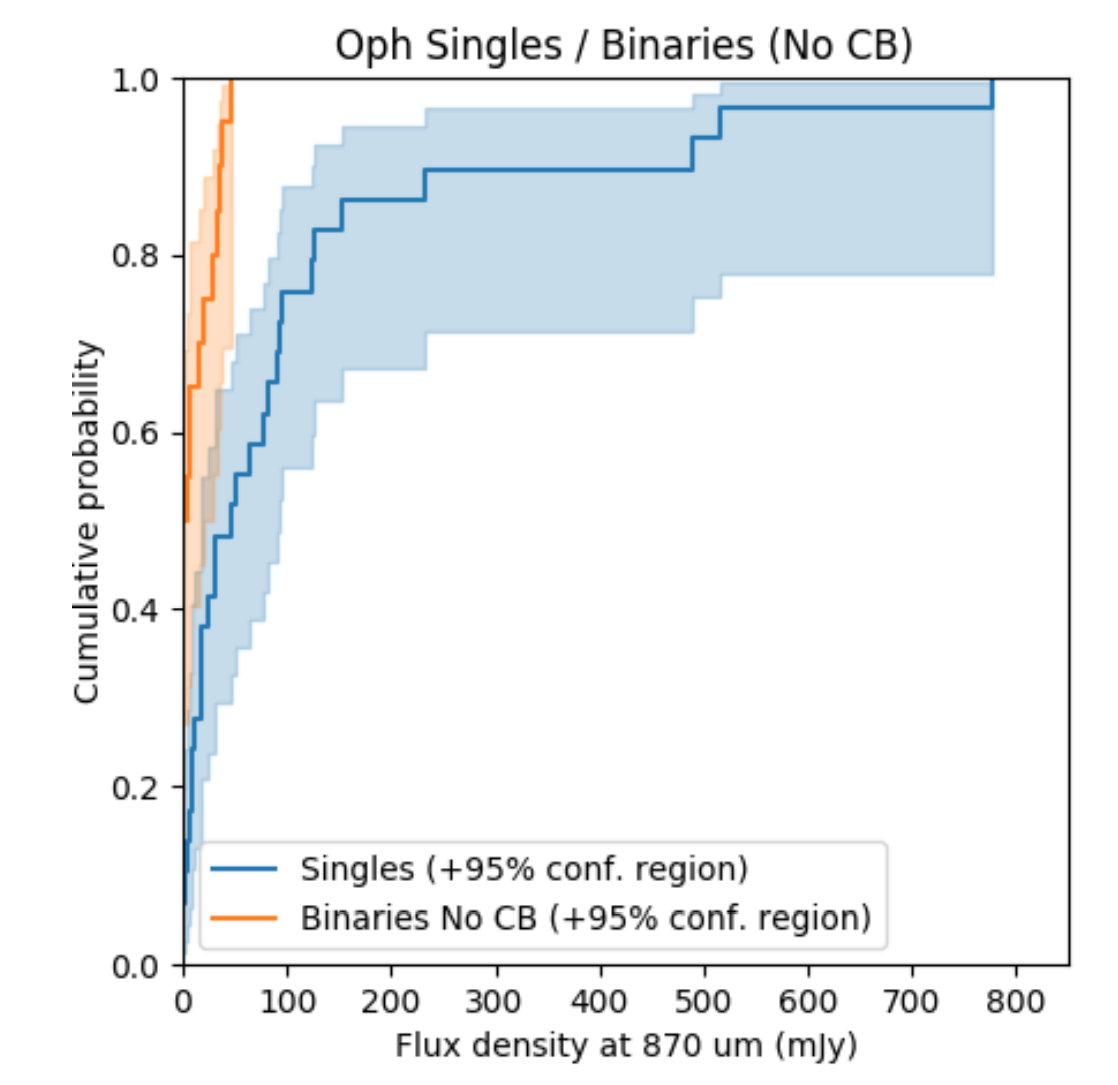
\includegraphics[width=0.5\linewidth]{cox17_rhoOph-singles-bins.png}}%
   \subcaptionbox{}{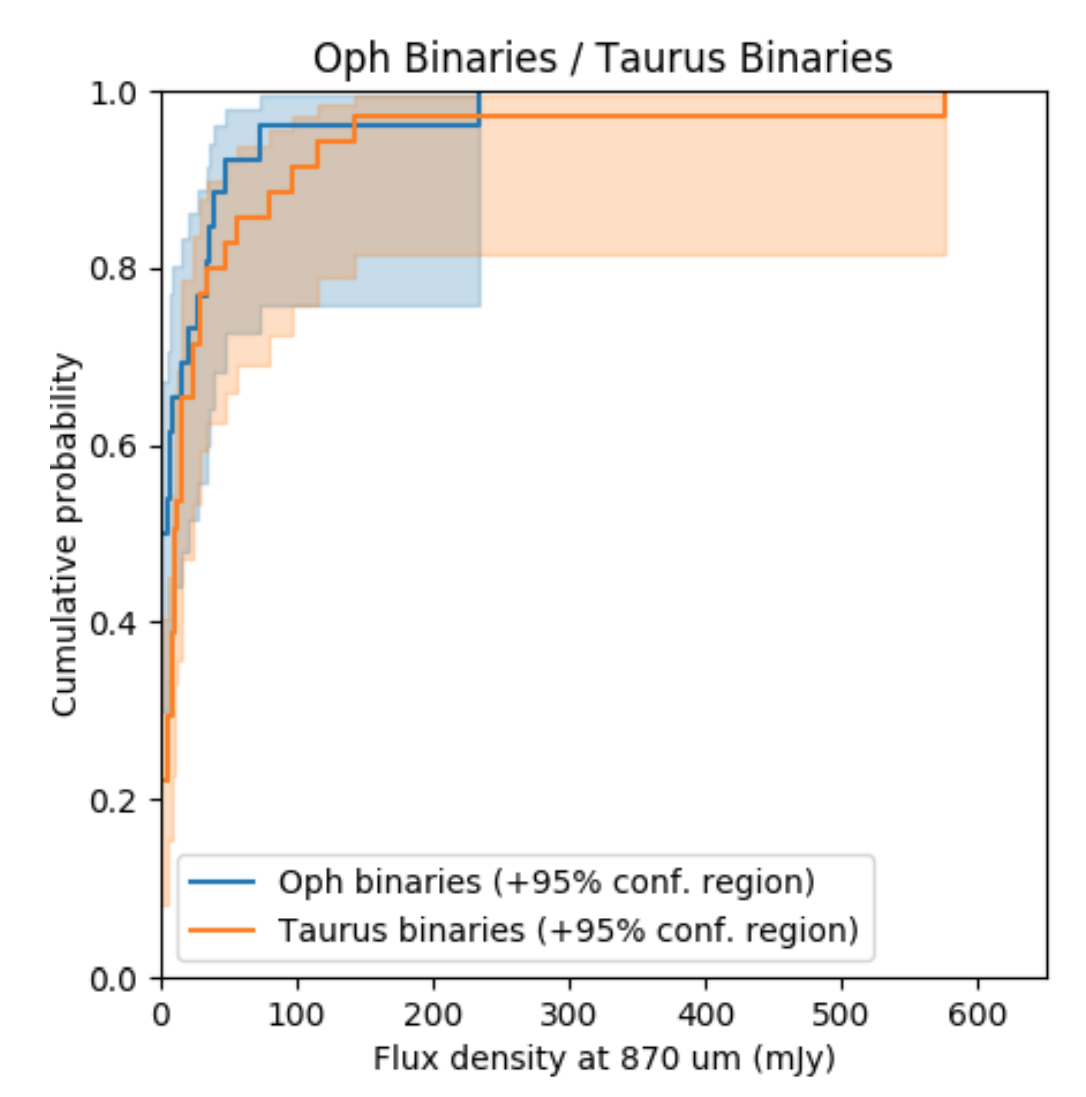
\includegraphics[width=0.5\linewidth]{cox17_taurus-rhhOph-bins.png}}%
   \hspace*{\fill}%
   \caption{\citet{Cox2017} showed that disks in binary systems (excluding circumbinary disks) in $\rho$ Ophiucus have systematically lower fluxes than both isolated disks in the region (\textit{left}) and disks in binaries in Taurus \citep[from][]{Rebull2012}.}
   \label{fig:rhoOph_binaries}
 \end{figure}


% REWORK: Is this redundant?
Comparing the this thesis's binary pair to these surveys, however, immediately shows that its disks are neither faint nor small, neither in comparison to the disks in those surveys or to the disks in the survey that it was a part of. However, this is not really out of line from the morphological patterns presented in the surveys above since, at 428 au, the disks' projected separation is enough to put them beyond the reach of the most significant mass and radius truncations that closer binaries undergo, and its large distance from $\theta^1$ Ori C likewise protects it.






\section{Chemical Structures}
% Chem modeling from Meredith
% Nomura, Henning, Ewine, Semmenov, Henning and Semminov Review on Disk Chem,

We now explore the chemical nature of protoplanetary disks. These disks have strong radial and vertical gradients in their temperatures, densities, and radiation fields, creating a wide range of chemistries. These chemistries can be broadly divided into inner- and outer-disk regimes, thanks to exponential radial temperature decay \citep{Dartois2003}. Inner disk temps are high and thus best suited to IR observations, while outer disks are cold and better suited to sub-millimeter observations. Because our investigation is rooted in ALMA data, we will review the outer disk here. Working with the basic building blocks of hydrogen, nitrogen, oxygen, and carbon and a wide diversity of temperature, density, turbulence, and radiation environments, disks are able to develop an array of molecules in their outer regions, each with its own characteristic formation conditions and emission signatures. Understanding disk chemistry is a process of knowing which of these signatures to look for and make sense of what they are telling us.


Since the disks form out of molecular clouds, the abundances found there should provide reasonable initial guesses for our disks' chemical abundances. \citet{Aikawa1999} showed these to be (for the molecules that we model) X$_{\hco}$ = $9 \times 10^{-9}$ and X$_{HCN}$ = $2 \times 10^{-8}$. However, since disks undergo complex chemical evolution, developing a parametric understanding of the chemical structure and evolution of protoplanetary disks guides our interpretation of data. Below is a brief overview of some of the efforts that have been made for this.


% Thanks to freeze-out and photodissociation, molecular abundances tend to be depleted by a factor of 5-100 in disks compared to the abundances found in the Taurus molecular cloud.


\begin{figure}[h]
  \includegraphics[width=\linewidth]{Aikawa1999_chem_process_co.png}%
  \caption{The chemical process leading to the generation of \hco and HCN \citep{Aikawa1999}. We immediately see that the generation of \hco is directly dependent on CO, while that same \hco molecule can then combine with N to yield the disk's HCN.}
  \label{fig:chem_magic}
\end{figure}

% \citet{Dutrey1997} first pointed out that molecular abundances were one to two orders of magnitude below molecular cloud levels in PPDs
\citet{Aikawa1997} were some of the first to apply time-evolving chemical networks to protoplanetary disks, describing a radial model of the effects of cosmic rays in the outer disk and how they can convert CO and N$_2$ (which together dominate the disk's initial composition) into more complex organics, including HCN, through chemically active ions (Fig. \ref{fig:chem_magic}). \citet{Aikawa1999} expanded on the work, modeling the evolution of molecular abundances in an accreting protoplanetary disk. They show that the timescale of this chemical evolution is dependent on the disk's ionization rate and the size distribution of the dust grains, increasing with lower ionization rates and/or larger grains and vice versa. As grains grow, HCN abundances are lowered by orders of magnitude, since they depend heavily on the grain surface recombination of \hco, which is significantly smaller in the case of larger grains. \citet{AikawaHerbst1999} and \citet{Aikawa2002} added a vertical dependence to the model, first with density and then with temperature, allowing a full ($r, z$) description of chemical evolution of a protoplanetary disk's temperature and density profiles and calculating the resulting interactions between the gas and dust, X-rays, and cosmic rays. They found that ionization in the mid-plane is driven by cosmic rays, while at significant heights from the midplane, X-rays from the central star also become a major source. These efforts yielded approximately radially constant distributions of \hco and HCN, with \hco presenting column densities about an order of magnitude above those of HCN (a reversal from the molecular cloud's conditions). This highlighted the role of ionization in protoplanetary disks and the need for a more complete description of the effects of high-energy radiation - both from the central star and cosmic rays, across a wide range of energies - on the evolution of their gas masses.


% REWORK: Maybe add some stuff about general abundance evolution?

% REWORK: Woooah nelly this sucks
In \citet{Fogel2011}, the authors show how strong radiation fields (i.e. from neighboring massive stars) will have the effect of amplifying the disk's natural CO-based photo-chemistry (already driven by the host star) and increase the size of the disk's warm gas layer. Additionally, the disk's dust evolution can affect the gas \citep{Fogel2011,Akimkin2013}, with grain growth and sedimentation leading to decreased UV shielding of the disk's inner layers and pushing the disk's molecular layer closer to the midplane. As the grains grow larger, their total surface area decreases, making gas-grain collisions less frequent. These interactions are crucial for the evolution of \hco (and, consequently, HCN), as \citet{Aikawa1999b} show. The decreased surface area also offers less attenuation of incoming rays, ultimately slowing molecular freezeout. This, in turn, leads to heightened column densities for many species, including CO and HCN.


\begin{figure}[t]
  \hspace*{\fill}%
  \subcaptionbox{CO abundances}{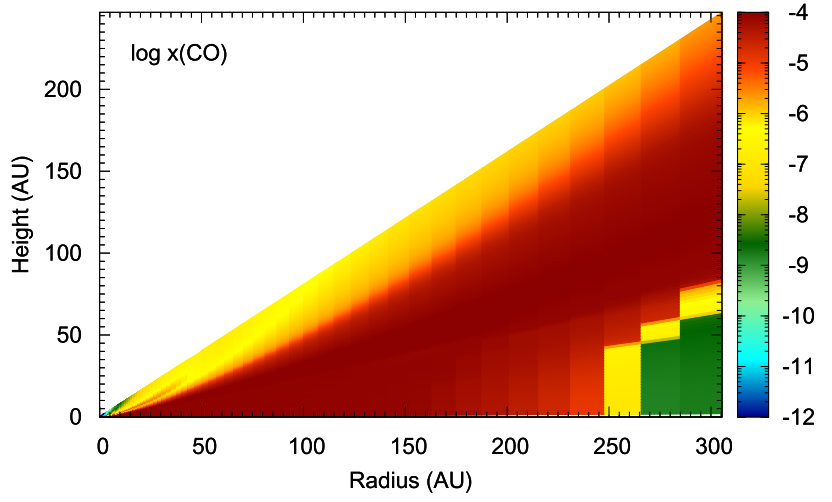
\includegraphics[width=0.33\linewidth]{walsh10_Xco.png}}%
  \subcaptionbox{\hco abundances}{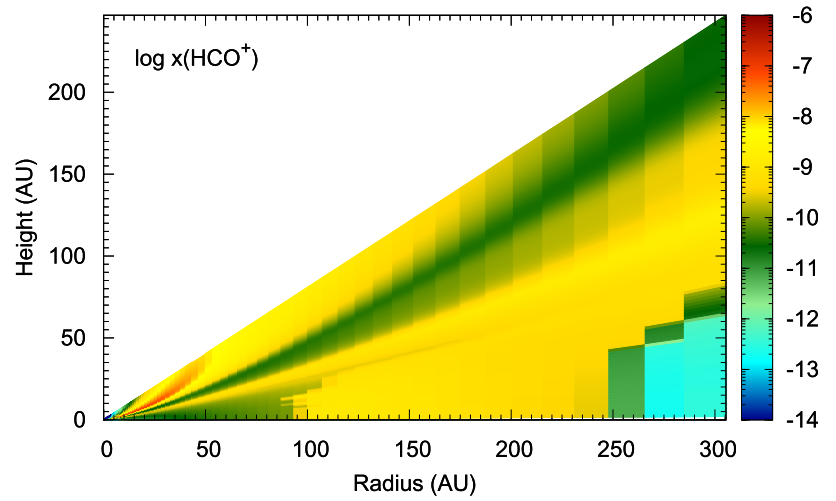
\includegraphics[width=0.33\linewidth]{walsh10_Xhco.png}}%
  \subcaptionbox{HCN abundances}{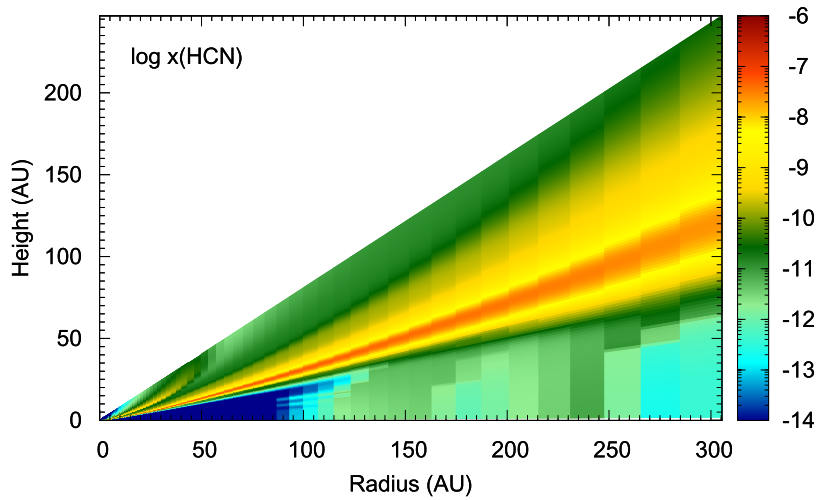
\includegraphics[width=0.33\linewidth]{walsh10_Xhcn.png}}\vfill%
  \subcaptionbox{CO abundances}{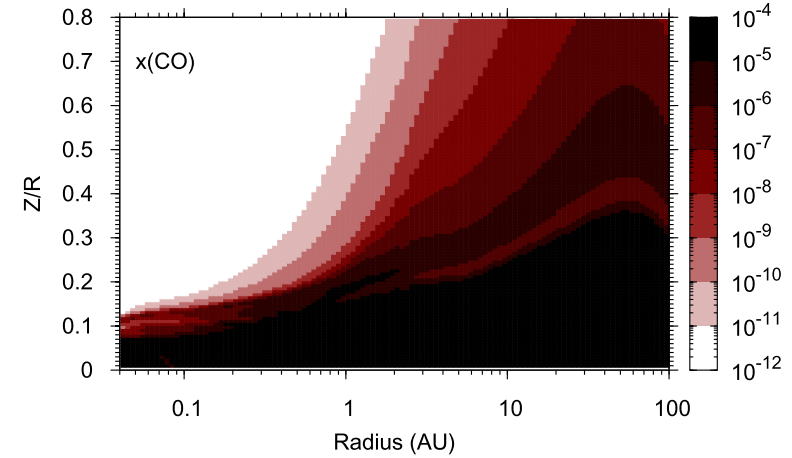
\includegraphics[width=0.33\linewidth]{walsh13_Xco.png}}%
  \subcaptionbox{\hco abundances}{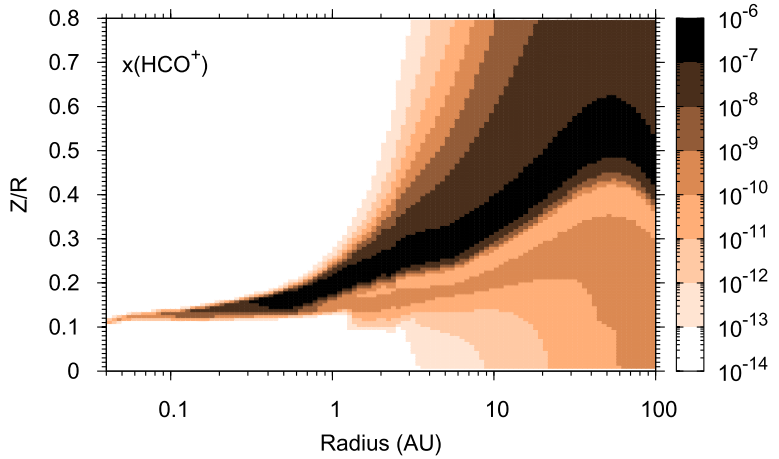
\includegraphics[width=0.33\linewidth]{walsh13_Xhco.png}}%
  \subcaptionbox{HCN abundances}{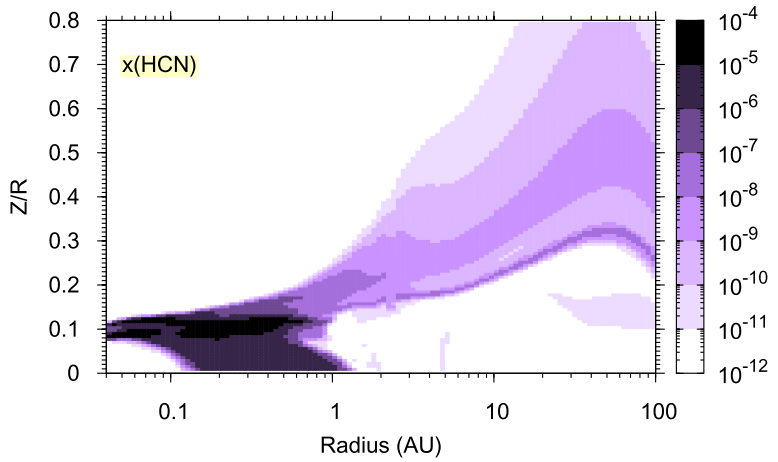
\includegraphics[width=0.33\linewidth]{walsh13_Xhcn.png}}%
  \hspace*{\fill}%
  \caption{Models showing radial and vertical distributions of CO, \hco, and HCN in a simulated disk around a T-Tauri star. The top row shows the profiles of isolated disks \citep{Walsh2010}, while the bottom row shows the profiles of disks being irradiated by a nearby O star \citep{Walsh2013}. Note that bottom row is on a log scale and only covers the inner 100 AU of the disk, while the top row is linearly scaled and shows a 300AU stretch.}
  \label{fig:walsh-abundance-profs}
\end{figure}




To study the effects of this ionization in anticipation of the arrival of ALMA, \citet{Walsh2010} developed radial and vertical chemical models for an isolated protoplanetary disk around a T-Tauri star, tracing molecular abundance distributions throughout the disk for molecules within ALMA's reach. They showed that log abundances in their models for \hco varied from $-8$ to $-12$, $-7$ to $-12$ for HCN, and $-4$ to $-9$ for CO, all of which are consistent with our fits. The authors then built on this model by adding functionality to model externally-driven UV and X-ray ionization \citep{Walsh2012} and applied it to the same disk system, this time with an O star nearby providing ionizing photons \citep{Walsh2013} and mapped molecular abundance distribution (see Fig.\ref{fig:walsh-abundance-profs}). The authors note that, in their externally photoionized disk, \hco column density increases by a factor of 6.3 relative to the isolated disk, whereas HCN and CO column densities remain constant through ionization. They also note that the ionized disks have much higher gas temperatures, T $\gg$ 50 K; this is consistent with the high temperatures that we see in our disks.
% This 6.3 increase would be useful if we had an estimation of what the \hco/HCN ratio would be in these two disks. They do have column density ratios in Walsh13; is it reasonable to say (I guess it would have to be in the case of optically thin emission) that col dens $\propto$ abundance? If that were the case then we'd be golden.


\citet{Cleeves2013,Cleeves2014} also modeled the radiation and ionization environment in these disks, developing models to compare the relative contributions of stellar UV, stellar X-rays, and cosmic rays (see Fig.\ref{fig:disk_ionization}). They found that stellar winds could disrupt cosmic rays and lowering their ionization rates by orders of magnitude. Their findings showed that \hco can trace high cosmic ray (CR) rates, with its abundances dropping significantly with decreased CR contributions, thanks to its precursor, CO, freezing out in regions where CRs are the primary energy source but deficient. They also note that \hco abundances can suffer from particularly high UV fluxes (from either Herbig host stars or high radiation environments), as CO can be photodissociated before having a chance to form \hco. %These influences allow \hco to trace the warm molecular ionization regions where CO is present in the gas.


% Henning2013 (Table 1): HCN traces photochemistry, HCO+ traces ionization
On the temperature side, we expect in an ideal disk to find $q=-0.5$ (recalling that the radial temperature structure is generally assumed to go as $T(r) \propto r^{q}$). This can be found by recalling that the energy that a star emits decays as something. Such a structure invokes the assumption of a smooth, consistent distribution of emitting material, so variations from that value indicate variations in the structure. Studies of individal disks (in low-mass SFRs) have largely been in line with this prediction \citep[e.g. ][, whose values range from -0.22 to -0.7]{Dartois2003,Panic2008,Panic2010,Hughes2008,Qi2003,Qi2004,Isella2007,Rosenfeld2012,Flaherty2015,Flaherty2017,Zhang2017,Flaherty2018}. In their study of another ONC proplyd, \citet{Factor2017} found that their HCN emission traced a moderately-high structure of $q=-0.18$, but that their \hco line showed $q=0.17$. \citet{Schwarz2016} note that a flatter, non-negative structure is to be expected when observing emission that originates from layers just above freeze out temperature in the disk.




\begin{figure}[t]
  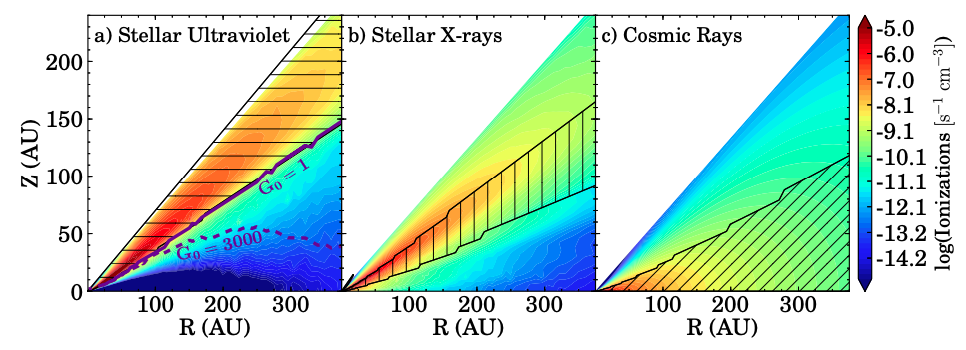
\includegraphics[width=\linewidth]{cleeves14_ionization_profiles.png}%
  \caption{Radiation contribution on a protoplanetary disk from stellar UV, stellar X-rays, and cosmic rays \citep{Cleeves2013}. \textit{(a)}: The $G_0 = 1$ contour represents the effects from a host-only UV field (i.e. an isolated star), while the $G_0 = 3000$ contour represents the effects of a UV field made up of both the host as well as from the interstellar radiation field. \cite{Fatuzzo2008} showed 3000 to be a typical value for $G_0$ in clusters. While the specific radiation field around these disks is unknown, \citet{Pabst2019} showed that they are in a region of $G_0 \geq 50$, indicating that they are likely in a field somewhere between the two contours. \textit{(b)}: Stellar X-rays are shown to dominate the inner regions of the disk, where the warm-molecular layer is and where HCN likely resides. Since d253-1536b is an actively accreting M star, it likely has X-ray flaring. \textit{(c)}:}
  \label{fig:disk_ionization}
\end{figure}







% Some references:
% - Observations and modeling of gaseous protoplanetary disks (2008): https://iopscience.iop.org/article/10.1088/0031-8949/2008/T130/014011/pdf
% - CHEMICAL NETWORK REDUCTION IN PROTOPLANETARY DISKS: https://arxiv.org/pdf/1901.04888.pdf
%     - Fig 4 predicts low (-12) X_HCO+
% - The chemistry of disks around T Tauri and Herbig Ae/Be stars: https://arxiv.org/pdf/1803.09450.pdf
%     - Shouldn't see differences in HCN/HCO+/CS abundances between disks around TT and HA/HB stars
% - AN ALMA SURVEY OF DCN/H13CN AND DCO+/H13CO+ IN PROTOPLANETARY DISKS: https://arxiv.org/pdf/1701.01735.pdf
%     - Seems cool but idk what's going on
% - MULTIPLE PATHS OF DEUTERIUM FRACTIONATION IN PROTOPLANETARY DISKS: https://arxiv.org/pdf/1803.02498.pdf
%     - How DCO+ gets formed. Interesting, but not critically relevant
% - Physical and chemical structure of planet-forming disks probed by millimeter observations and modeling: https://arxiv.org/pdf/1402.3503.pdf
%     - A nice 2014 review, but not sure what to take away from it
% - The first multi-dimensional view of mass loss from externally FUV irradiated protoplanetary discs (2019): https://arxiv.org/pdf/1903.03644.pdf
% - Stellar disk destruction by dynamical interactions in the Orion Trapezium star cluster (2015): https://arxiv.org/pdf/1511.08900.pdf
% - External photoevaporation of protoplanetary discs in Cygnus OB2: linking discs to star formation dynamical history (2019): https://arxiv.org/pdf/1902.04586.pdf
% - Slideshow from Oberg: https://www.cfa.harvard.edu/sma/events/smaConf/posters/images/Oberg_SMA_archive.pdf
%   - p. 17: chemical depletion of CO

% Some more references:
% - Aikawa1999: https://iopscience.iop.org/article/10.1086/307400/pdf
% - Aikawa2002: https://arxiv.org/pdf/astro-ph/0202060.pdf
% - Semenov2011: Review of disk chem: https://arxiv.org/pdf/1107.4513.pdf
% - HenningSemenov2013: Bigger review of disk chem: https://pubs.acs.org/doi/pdf/10.1021/cr400128p
% - Akimkin2013: Modeling disk chem with dust: https://arxiv.org/pdf/1302.1403.pdf
% - Bergin+: Chem. Ev. of PPDs: http://www.ita.uni-heidelberg.de/research/klessen/internal/pp5/sec8-1.pdf
% - Harada2017: Grain growth effects on abundances: https://iopscience.iop.org/article/10.3847/1538-4357/aa602f/pdf
% - Dutrey2014: Phys. and Chem. Str. of PPDs: https://arxiv.org/pdf/1402.3503.pdf



% REWORL: Fix the Aikawa ref in the table, think bout whether it should be there. Also
% \begin{table}[ht!]
%   % \centering
%   \begin{threeparttable}
%     \caption{Disk Parameter List}
%     \label{table:comparisons}
%     \renewcommand{\arraystretch}{1.2}
%     \begin{tabular}{l l l c c c }
%       \toprule \toprule
%       %\multirow{2}{*}{Parameter} & \multirow{2}{*}{Disk A}    & \multicolumn{2}{c}{Disk B} \\
%       Reference                             & Source     & Line          & $q$ & log X$_\text{mol}$  & Atms. Temp (Measured Radius)\\
%       \midrule %\midrule
%       \multirow{3}{*}{This study}           & d253-1536a & \hco(4-3)      & $0.66$  & $-7.96$         & 151 (150 au) \\
%                                             & d253-1536a & HCN(4-3)       & $0.72$  & $-7.62$         & 140 (150 au) \\
%                                             & d253-1536a & CO(3-2)\tnote{a} & $0.40$  & $[-4]$        & 1 (150 au) \\
%       \hline
%       \multirow{3}{*}{\cite{Factor2017}}    & d216-0939  & \hco(4-3)      & $0.17$  & $-10.08$        & 190 (150 au) \\
%                                             & d216-0939  & HCN(4-3)       & $-0.18$ & $-6.7$          & 19 (150 au) \\
%                                             & d216-0939  & CO(3-2)        & $-0.33$ & $[-4]$          & 70 (150 au) \\
%       % \hline
%       % \multirow{3}{*}{\cite{Aikawa1999}}& Molecular Cloud  & \hco(4-3)      & $ [-]$  & $-10.08$        & 190 (150 au) \\
%       %                                   & Molecular Cloud  & HCN(4-3)       & $ [-]$ & $-6.7$          & 19 (150 au) \\
%       % \hline
%       % \multirow{2}{*}{\citet{Flaherty2015}} & HD163296   & CO(3-2)        & $-0.22$ & $[-4]$          & 94 (150 au)  \\
%       %                                       & HD163296   & CO(2-1)        & $-0.27$ & $[-4]$          & 79 (150 au) \\
%       % \hline
%       % \multirow{2}{*}{\citet{Dartois2003}}  & DM Tau     & $^{13}$CO(2-1) & $-0.30$   & $[-5.79]$       & 22 (100 au)  \\
%       %                                       & DM Tau     & C$^{18}$O(2-1) & $-0.30$   & $[-5.79]$       & 35 (100 au) \\
%       % \hline
%       % \multirow{2}{*}{\citet{Chapillon2013}}& LkCa 15    & HCN(1-0)      & $-0.55$   & $[-]$          & 7   (300 au) \\
%       %                                       & DM Tau     & HCN(1-0)       & $-0.0$   & $[-]$          & 36  (300 au)  \\
%       % \multirow{2}{*}{\citet{Chapillon2018}}& CQ Tau     & CO(2-1)       & $-0.7$    & $[-]$          & 150 (100 au) \\
%       %                                       & MWC 758    & CO(1-0)       & $-0.6$    & $[-]$          & 24  (100 au)  \\
%       % \hline
%       % \citet{Rosenfeld2012}\tnote{b}        & V4046 Sgr  & $^{12}$CO(2-1) & $-0.63$ & $[-4]$           & -  \\
%       % \hline
%       % % \citet{Dutrey2014}        & GG Tau A  & Continuum & $-1.1$ & NA          & 13.8  \\
%       % % \hline
%       % \citet{Flaherty2017}\tnote{c}         & HD163296   & DCO$^+$(3-2)   & $[-2.22]$ & $-10.79$      & [94]  \\
%       % \hline
%       % \citet{Zhang2017}                     & TW Hya     & $^{13}$C$^{18}$O(3-2), C$^{18}$O(3-2)  & $-0.47$ & -7.96 & 151  \\
%       % \hline
%       % \citet{Flaherty2018}\tnote{d}         & TW Hya     & CO(6-5, 3-2, 2-1) & $-0.46$ & $[-4]$       & 31  \\
%       % Charlie Qi for this, and other mol. line stuff
%       % French group (Dutrey, Dartois etc) (Simon et al (2010ish))
%       % Panic 2008ish
%       % Isella et al
%       \bottomrule
%     \end{tabular}
%     \begin{tablenotes}\footnotesize
%       \item[*] Values in [brackets] were fixed during fitting.
%       \item[**] Since there is not a convention about whether a negative value of $q$ indicates a radially decreasing or increasing temperature structure (in other words, whether or not $q$ is implicitly negative), some of these values have the opposite sign of the value reported in their article. When this is the case, it indicates that, in that original paper, atmospheric temperature was defined such that T$_\text{atms} \propto r^{-q}$. In our work, and in all the values given here, it is the case that T$_{atms} \propto r^{q}$, meaning that a negative value of $q$ leads to temperature decreasing with radius.
%       \item[a] This result is being presented for completeness (and to allow for the chance that something changes dramatically in coming runs REWORK), but since its T$_{atms}$ clearly got stuck, it is not a useful result for comparison and will not be discussed.
%       \item[b] \cite{Rosenfeld2012} didn't fit for tatms
%       \item[c] In \citet{Flaherty2017}, they fit three rings, and consequently have three slightly different values for each parameter. The values reported here are for their middle ring, although the three do not vary significantly from one another. Additionally, T$_{atms}$ and $q$ were fixed at values found for CO(3-2) in \citet{Flaherty2015}, and only X$_\text{mol}$ was fit for.
%       \item[d] \citet{Flaherty2018} developed several models, with different morphological structures. The results presented here are drawn from their simplest (fiducial) model.
%     \end{tablenotes}
%   \end{threeparttable}
% \end{table}
% TO ADD:
% Dutrey 2014: Disks in CG Tau: https://www.nature.com/articles/nature13822#abstract













\section{Implications}
% - The thing that’s really missing from the discussion is a conversation about what this all means.  *Why* might the similarities/differences between your disk and Sam’s, or your disk and the ones in low-mass SFRs exist?  I think you will be able to write it a lot better once you have expanded your reading beyond just Catherine Walsh’s modeling.  What factors do the modelers predict should affect the chemistry of these disks?  How are these factors related to environment?  To what extent might they be influenced by binarity?  



% MASS DISCUSSION
With this context, how do now we make sense of our current observations and fits? Our results show a wide (428 au separation) binary pair of stars with disks that are massive\footnote{Although this mass is, of course, still handicapped by the assumptions about gas/dust ratios} and radially large (both compared to other disks in the ONC and disks in binaries in Taurus and $\rho$ Ophiucus). The two disks have appreciably different chemistries, and are physically interacting, as shown by the HCN residuals.


Since our disk model produces a single, flat relative abundance for each molecule across the disk, we are inherently unable to resolve the level of detail presented in the models. However, we may tentatively recognize their predictions to inform how we interpret our results. According to \citet{Walsh2013}, \hco is a tracer of cold, dense material and is generally more abundant in the outer midplane, whereas HCN follows warmer material closer in to the disk's center (since it is non-volatile, it freezes out more easily). Their models predict that, in an isolated disk, the line strength (in units of mJy \kms) ratio of HCN/\hco should be 27.1/54.1 (0.50), while in an irradiated disk it is 71.9/86.9 (0.83). Using the line strengths that we reported in \S\ref{chap:results}, we find in disk A's ratio to be 0.69/4.15 (0.17) and disk B's at 0.26/0.80 (0.33), significantly lower even than the isolated disk. Assuming that these are physically-driven results, they could also help explain the unexpectedly high $q$ value that our MCMC walkers settled on, as, in agreement with the Walsh prediction above, these would imply that \hco is extremely abundant and that that mass is stored in the disks' outer reaches, forcing the temperature profile to flip to compensate for the flux out there since the abundance is forced to remain flat. This is also consistent with the \citet{Schwarz2016} observation that a high $q$ value would reflect emission from layers just above freeze out, since that is where \hco would be found.


This casts our interpretation of the abundances in an interesting light. It is a bit uncertain to what degree they should be trusted since, if the above interpretation is correct, then a flat abundance structure is likely a bad approximation. However, we still do see interesting features in these numbers which are worth exploring. As shown in \S\ref{chap:results}, disk A's ratio of log abundances between HCN and \hco, X$_\text{HCN}$/X$_\text{\hco}$, is 8/8.2, while disk B's is 9.9/9.8. The fact that both disks present a nearly identical ratios but that the abundances are separated by nearly two-orders of magnitude seems to reflect some difference in structure between the two disks.

One immediate explanation could be found by recalling that the two disks are hosted by very different stars: d253-1536a is an F or G star, and nearly nine times as massive as d253-1536b, an accreting M-star. It is possible that one star could have stronger emission at an energy that affects both molecules equally, either depleting or enhancing both together and yielding the observed discrepancy. Another way of increasing abundances, as described above, is through dust grain growth/dust depletion, as the resulting decrease in the dust's total surface area leads to both decreased shielding and decreased area for gas-grain interactions and slowing molecular freeze out. This relative dust mass can be approximated with a quick density calculation of M$_\text{dust}/r$, which for disk A yields $78/341$ = 0.23 M$_\text{Jup}$/au and 30/148 = 0.20 M$_\text{Jup}$/au for disk B. However, since these values are quite close and given the significant uncertainties in the mass measurements, a more nuanced study would be needed to follow this approach. Another dust-related explanation could be that bodies too large for ALMA to see (from pebbles and boulders to planets and planetesimals) may be depleting one disk's gas mass, as proposed by \citet{Miotello2016}. Whether this would be a chemically-selective depletion (i.e. whther or not it would affect both \hco and HCN evenly) is unclear, but should be considered a possibility.
% what is the effect of a planet on disk chemistry?

% Andrews, Tripathi, maybe someone else on mass/radius dust ratios
% 78/341 = 0.23
% 30/148 = 0.20

A less probable but still fascinating possibility is that these disks did not form together. \citet{Williams2014} posit that wide binaries (systems with separations $\geq$ 300 au) such as this one do not form in the same initial cloud structures. If this were the case, then it might be reasonable to expect each disk to reflect different chemistries of the regions in which each star formed. However, binary capture is rare, as a third star is required for this proces to create a bound pair \citep[e.g. ][]}{Mansbach1970}, and it is unclear whether the local stellar environment shows history of such an event. It is also unclear how the binary's stellar mass ratio - around 9:1 - would affect the capture process, as such captures usually involve mass ratios closer to unity.

% REWORK: Re the footnote: "Hm, I’m not sure either, but I would take a look at Robert Harris’s PhD thesis papers on binaries with the SMA as a starting point — check his intro and discussion for relevant references.  Could also check the more recent Akeson/Jensen papers on binaries with ALMA for some relevant intro/discussion material.  Would be good to expand upon this point in the discussion."




% Regardless of what the primary driver of this chemical asymmetry between the two disks, the radiation environment in which these disks exist is a fascinating one, thanks to the unique combination of a relatively high-mass star (d253-1536a), an heavily-accreting M-star (d253-1536b), and, even though they are far from the Trapezium cluster, \citet{Pabst2019} recently showed that marginal ionization from Trapezium is still present well past M43 (see Fig.\ref{pabst2019_onc_ionization}).
% \begin{figure}[h]
%   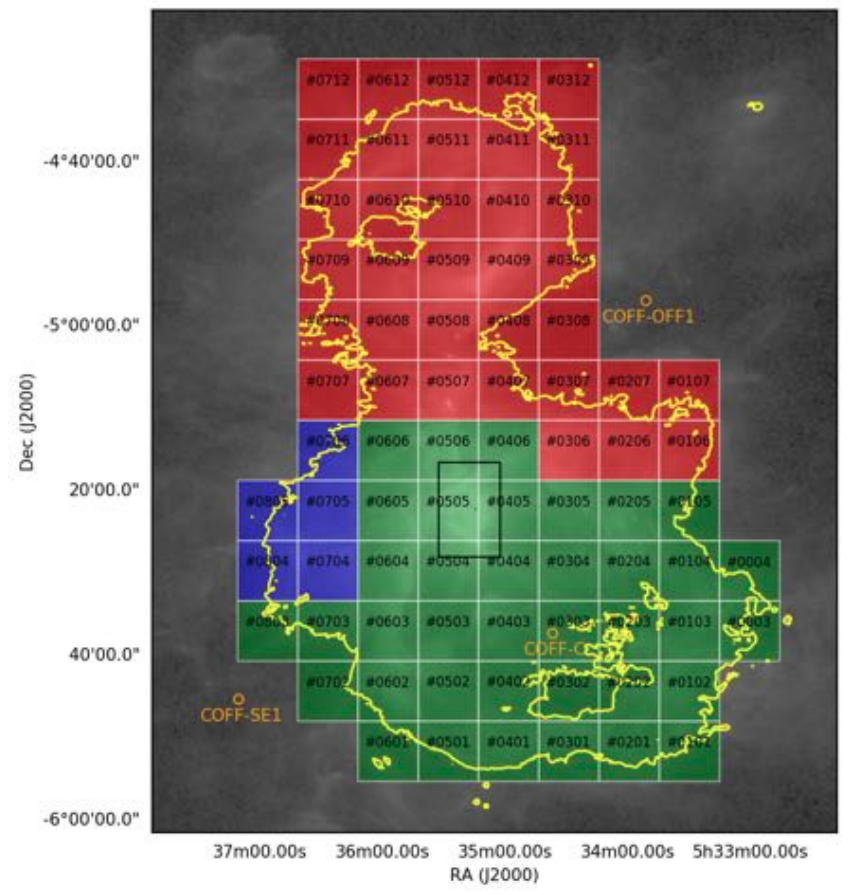
\includegraphics[width=\linewidth]{pabst2019_onc_ionization.png}%
%   \caption{blah blah}
%   \label{fig:pabst2019_onc_ionization}
% \end{figure}







% The End
